\begin{sagesilent}
import numpy as np

def stampa_dati(wa, header):
  s = r"\begin{tabular}{c*{" + "%d" % (len(wa.dtype)-1)
  s += r"}{|c}}"
  s += "%s \\\\" % (header)
  s += r"\midrule"
  for i in range(0, len(wa)):
    a = ["%s" %x for x in wa[i]]
    s += "%s \\\\" % join(a, "&")
  s += r"\end{tabular}"
  return s
\end{sagesilent}



\chapter{C1}

L'obiettivo del nostro esperimento è misurare la validità della legge di Ohm per varie configurazioni di un circuito. 

Al fine di misurare corrente e potenziale, colleghiamo al nostro circuito due multimetri digitali. Il primo, che ha la funzione di voltmetro, lo poniamo ai capi della nostra resistenza collegato in parallelo; il secondo, in modalità amperometro, è posto in serie subito dopo la resistenza. 

Di seguito, gli strumenti con la loro precisione:
\begin{itemize}
\item Voltmetro (multimetro portatile)
\item Amperometro (multimetro da banco)
\item Generatore da banco, resistenza interna ignota.
\end{itemize}


\section{Resistenze}

Ricaviamo, tramite  il fit della funzione $V=R*I$ dove R è parametro da stimare, il valore di due resistenze ignote. Di seguito i dati del circuito 1 e del circuito 2. 


\begin{center}
\begin{tabular}{*{4}{c}}
Corrente1($nA$) & Potenziale1($mV$) & Corrente2($nA$) & Potenziale2($mV$)\\
\midrule
396 & 201 & 3043 & 207\\
512 & 261 & 3667 & 250\\
706 & 360 & 4703 & 319\\
890 & 454 & 6365 & 432\\
1126 & 574 & 8984 & 609\\
1242 & 633 & 12326 & 836\\
1557 & 794 & 16898 & 1145\\
1812 & 925 & 340 & 24\\
1971 & 1005 & 725 & 50\\
2290 & 1168 & 966 & 66\\
2524 & 1286 & 1595 & 108\\
2850 & 1454 & 1822 & 124\\
3116 & 1589 & 2160 & 146\\
3407 & 1737 & 2302 & 157\\
3883 & 1980 & 2584 & 176\\
4229 & 2157 & 3100 & 211\\
4598 & 2344 & 3370 & 229\\
5072 & 2586 & 4036 & 274\\
5505 & 2807 & 4348 & 295\\
5820 & 2967 & 4596 & 312\\
6257 & 3191 & 4894 & 332\\
6738 & 3436 & 5578 & 379\\
7521 & 3835 & 6613 & 449\\
7880 & 4018 & 6963 & 473\\
8493 & 4331 & 7371 & 500\\
8852 & 4514 & 7864 & 533\\
9135 & 4658 & 8603 & 584\\
9431 & 4809 & 9066 & 615\\
9720 & 4957 & 9667 & 656\\
9972 & 5085 & 10816 & 733\\

\end{tabular}
\end{center}


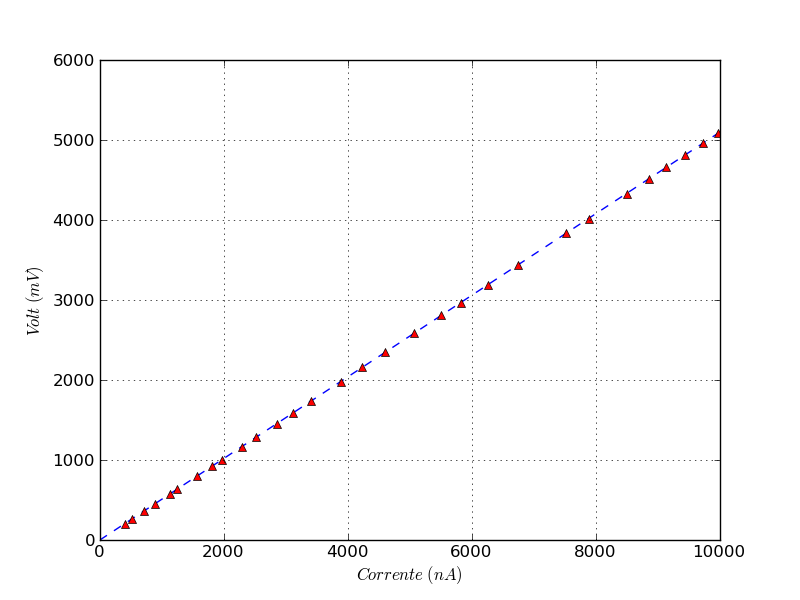
\includegraphics[scale=0.75]{grafici/C1/res1.png}
\

Parametri trovati dal fit: \
$R= 5099 \pm 0.3 \ \Omega$

$q = -0.113 \pm 0.147\ mV$


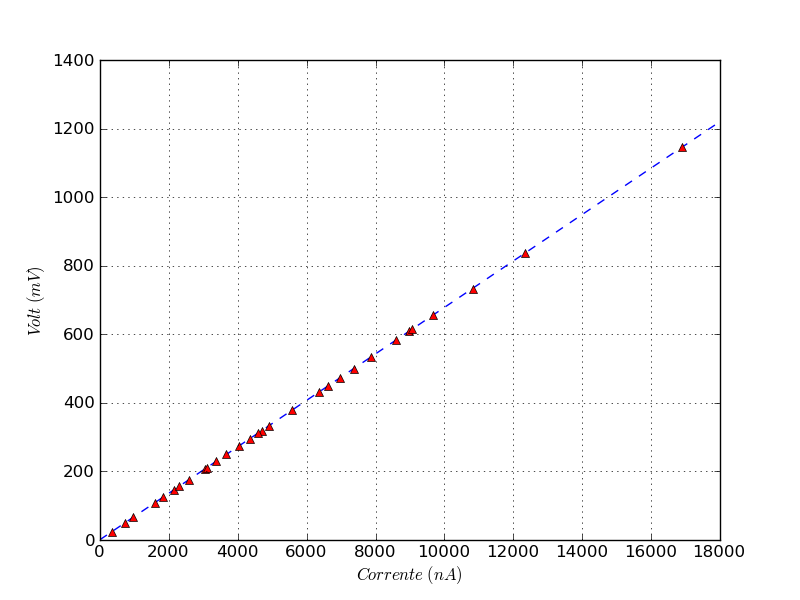
\includegraphics[scale=0.75]{grafici/C1/res2.png}

$R = 677 \pm 2.02\cdot 10^{-1} \Omega$

$q = 0.72 \pm 1.35\cdot 10^{-1} \ mV $
\

\section{Serie e Parallelo}

L'incertezza sulla misura è quello dello strumento. Nel caso dell'amperometro $\sigma_a = 0.0001\ A$ , per il voltmetro
$sigma_v = 0.001\ V$ per le misure in serie, e $sigma_v = 0.01\ V$ per le misure in parallelo.
\\

\begin{sagesilent}
 
 import numpy as np
 import matplotlib.pyplot as plt
 from scipy import odr

 cs = np.recfromcsv("dati/c1-serie.csv",delimiter="\t")
 
 cp = np.recfromcsv("dati/c1-parallelo.csv",delimiter="\t")

 #Errori presi da risoluzione strumento
 yerr1=0.001
 yerr2=0.01
 xerr=0.0001
 
 def fu(P,x):
    return P[0]*x + P[1]

 mymod = odr.Model(fu)
 mydata = odr.RealData(cs['i'], cs['v'], sy=yerr1)
 myodr = odr.ODR(mydata, mymod, beta0=[50, 0.1], maxit=1000)
 myout = myodr.run()
 myout.pprint()
 
 mymod = odr.Model(fu)
 mydata = odr.RealData(cp['i'], cp['v'], sy=yerr1)
 myodr = odr.ODR(mydata, mymod, beta0=[50, 0.1], maxit=1000)
 myout = myodr.run()
 myout.pprint()

 plt.clf()
 plt.subplot(211)
 plt.errorbar(cs['i'],cs['v'],yerr1,xerr,fmt='b.')
 plt.ylabel("Potenziale V")
 plt.grid(True)
 
 plt.subplot(212)
 plt.errorbar(cp['i'],cp['v'],yerr2,xerr,fmt='r.')
 plt.grid(True)
 plt.ylabel("Potenziale $V$")
 plt.xlabel("Corrente $A$")
 plt.savefig("grafici/C1/c1B.png",dpi=300)
 
\end{sagesilent}


\sagestr{stampa_dati(cs, r"Potenziale (V) & Corrente (A)")}
\

\sagestr{stampa_dati(cp, r"Potenziale (V) & Corrente (A)")}

\includegraphics[scale=0.75]{grafici/C1/c1B.png}

Il primo grafico mostra l'andamento del potenziale in funzione della corrente per un circuito dotato di due resistenze in serie da $1297\ \Omega$
Dal fit ricaviamo un valore di $2117 \Omega$, che ben si avvicina al valore teorico $R_{eq}=R_1+R_2= 2594\ \Omega$.

Il secondo grafico, sono invece le due medesime resistenze in parallelo. Dal fit si ricava una resistenza equivalente di
$R = 604 \Omega$, che ben si accorda con il valore teorico $R_{eq} = \frac{R_1 \cdot R_2}{R1+R2}=648\ \Omega$.

Gli errori sui fit non sono stati riportati perchè trascurabili. 
\\

\section{Resistenza interna dei multimetri}
Misuro la resistenza interna del voltometro, mantenendo costante la ddp a $14.5\ V$ e variando la resistenza all'interno del circuito. 
Il voltmetro è in parallelo al circuito, perciò $R_i$:

$$R_i = \frac{RV}{RI-V} $$

dove R è la resistenza variabile, I la corrente nel circuito e $V= 14.5\ V$

\begin{center}
\begin{tabular}{*{2}{c}}
Resistenza $M\Omega$ & Corrente $nA$\\
\midrule
7&      36\\
9&      32\\
10& 30\\
11&     29\\
12&     28\\
13&     27\\
14&     26\\
15&     26\\
16&     25\\
17&     24\\

\end{tabular}

\end{center}
La resistenza risulta $9.20 \pm 0.27 \ M \Omega$.


Misuriamo la resistenza interna dell'amperometro, che è collegato in serie al circuito. 

$$R_i = \frac{V-RI}{I}$$

In questo caso, R è fissato ($R=0.5 \Omega$) e sono V e I a variare
\begin{center}
\begin{tabular}{*{2}{c}}
Volt $mV$ & Corrente $nA$\\
\midrule
22&      1769\\
40&      3271\\
60&      5047\\
105&     8938\\
133&     11201\\
142&     12021\\
164&     13882\\
174&     14745\\
208&     17604\\
232&     19671\\



\end{tabular}
\end{center}

La resistenza interna risulta $11.42 \pm 0.45 \Omega$

Colleghiamo una piccola lampada a filamento al circuito, e verifichiamo che il suo comportamento resistivo non segue la legge di Ohm. 

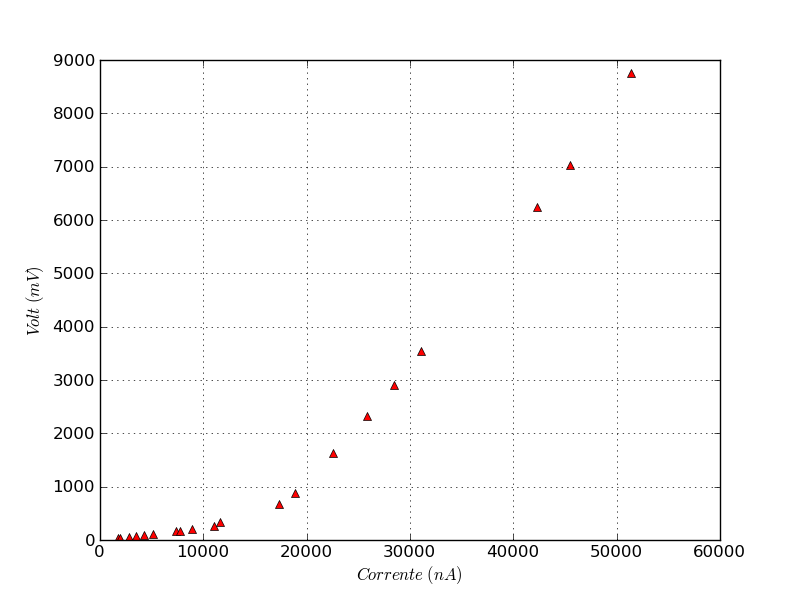
\includegraphics[scale=0.75]{grafici/C1/lampa.png}

La lampadina ha un comportamento non-ohmico nel momento in cui il filamento si scalda sufficientemente e inizia ad emettere luce ($500mV$).


\section{Partitore resistivo}
Il partitore di corrente è un circuito utilizzato per calcolare la corrente elettrica che scorre attraverso un'impedenza o attraverso un circuito quando esso viene connesso in parallelo con un'altra impedenza.
Nel nostro caso, stiamo analizzando un partitore resistivo. 

\subsection{Situazione senza carico}
\begin{center}
\begin{tabular}{*{2}{c}}
$V_{in}$ & $\frac{V_{in}}{V_{out}}$\\
\midrule
329.0 & 0.5015 \\
493.0 & 0.501 \\
544.0 & 0.5018 \\
618.0 & 0.5016 \\
667.0 & 0.5007 \\
776.0 & 0.5 \\
803.0 & 0.5006 \\
927.0 & 0.5005 \\
1078.0 & 0.5 \\
1285.0 & 0.4996 \\
\end{tabular}

\end{center}


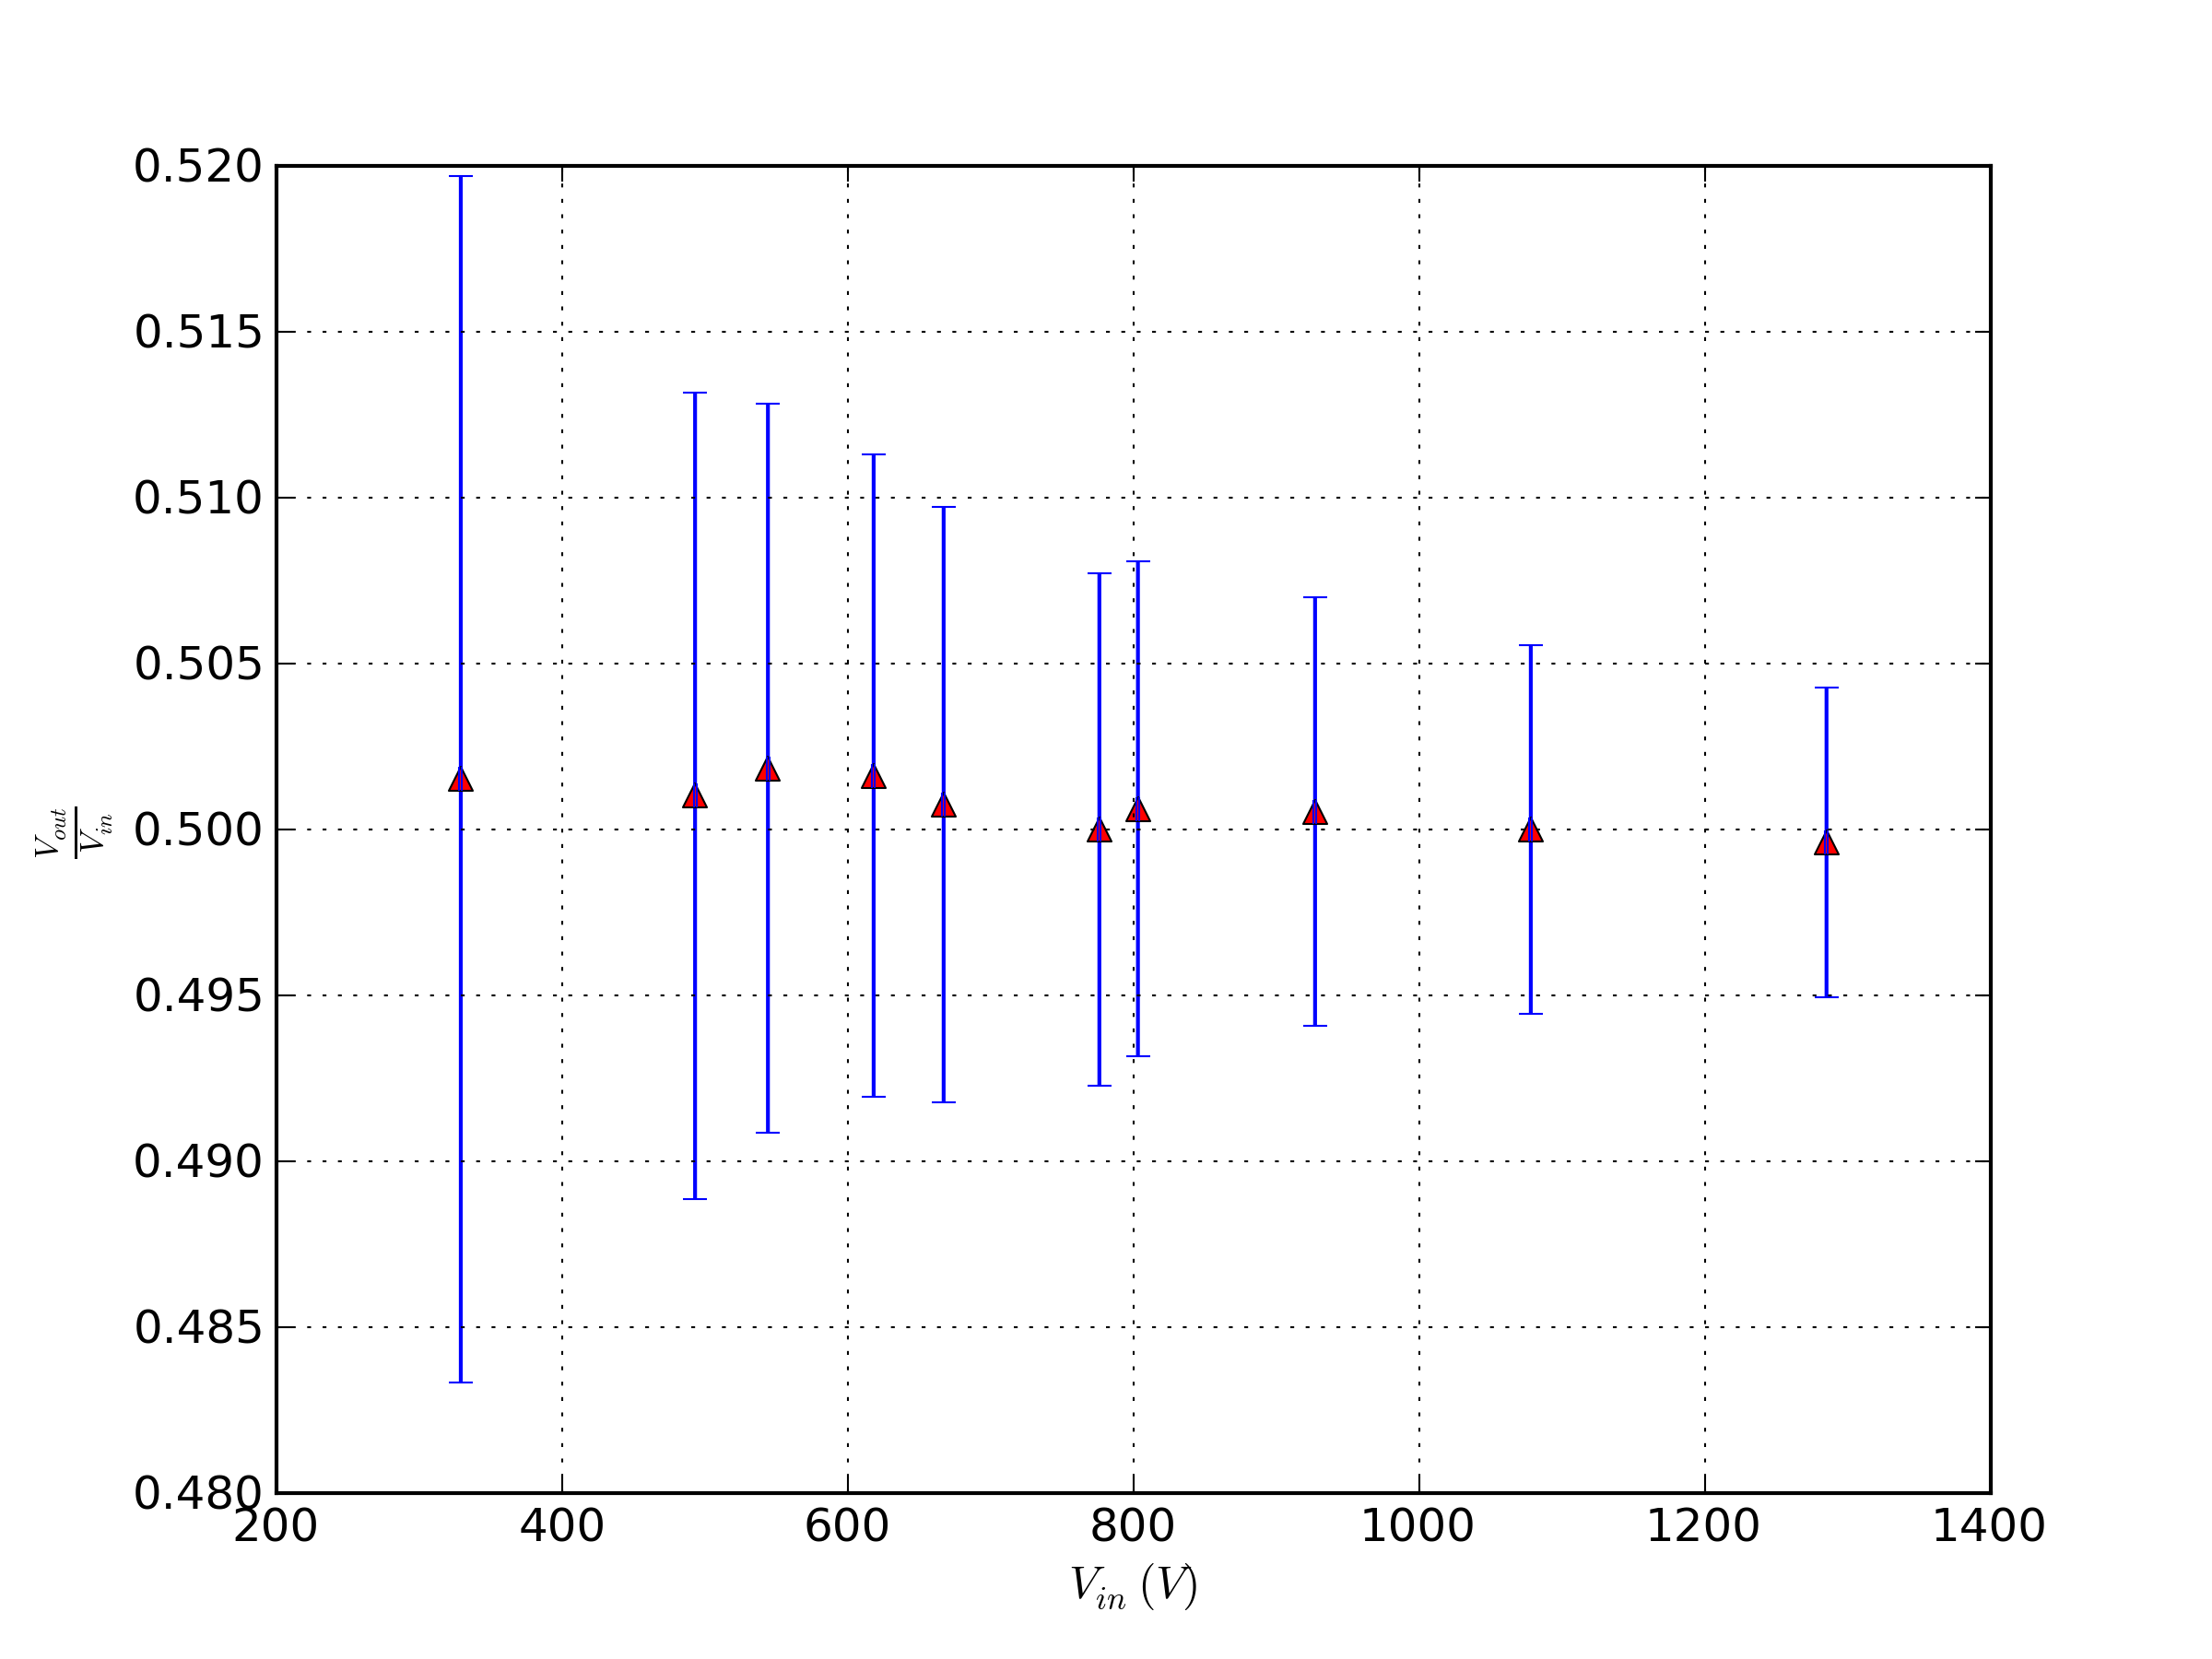
\includegraphics[scale=0.75]{grafici/C1/part11.png}

\subsection{Situazione con carico}
\begin{center}

\begin{tabular}{*{2}{c}}
$V_{in}$ & $\frac{V_{in}}{V_{out}}$\\
\midrule
220.0 & 3.1 \\
276.0 & 3.1051 \\
302.0 & 3.1126 \\
410.0 & 3.1073 \\
511.0 & 3.1115 \\
559.0 & 3.1055 \\
624.0 & 3.109 \\
752.0 & 3.109 \\
906.0 & 3.1093 \\
1036.0 & 3.111 \\
\end{tabular}

\end{center}
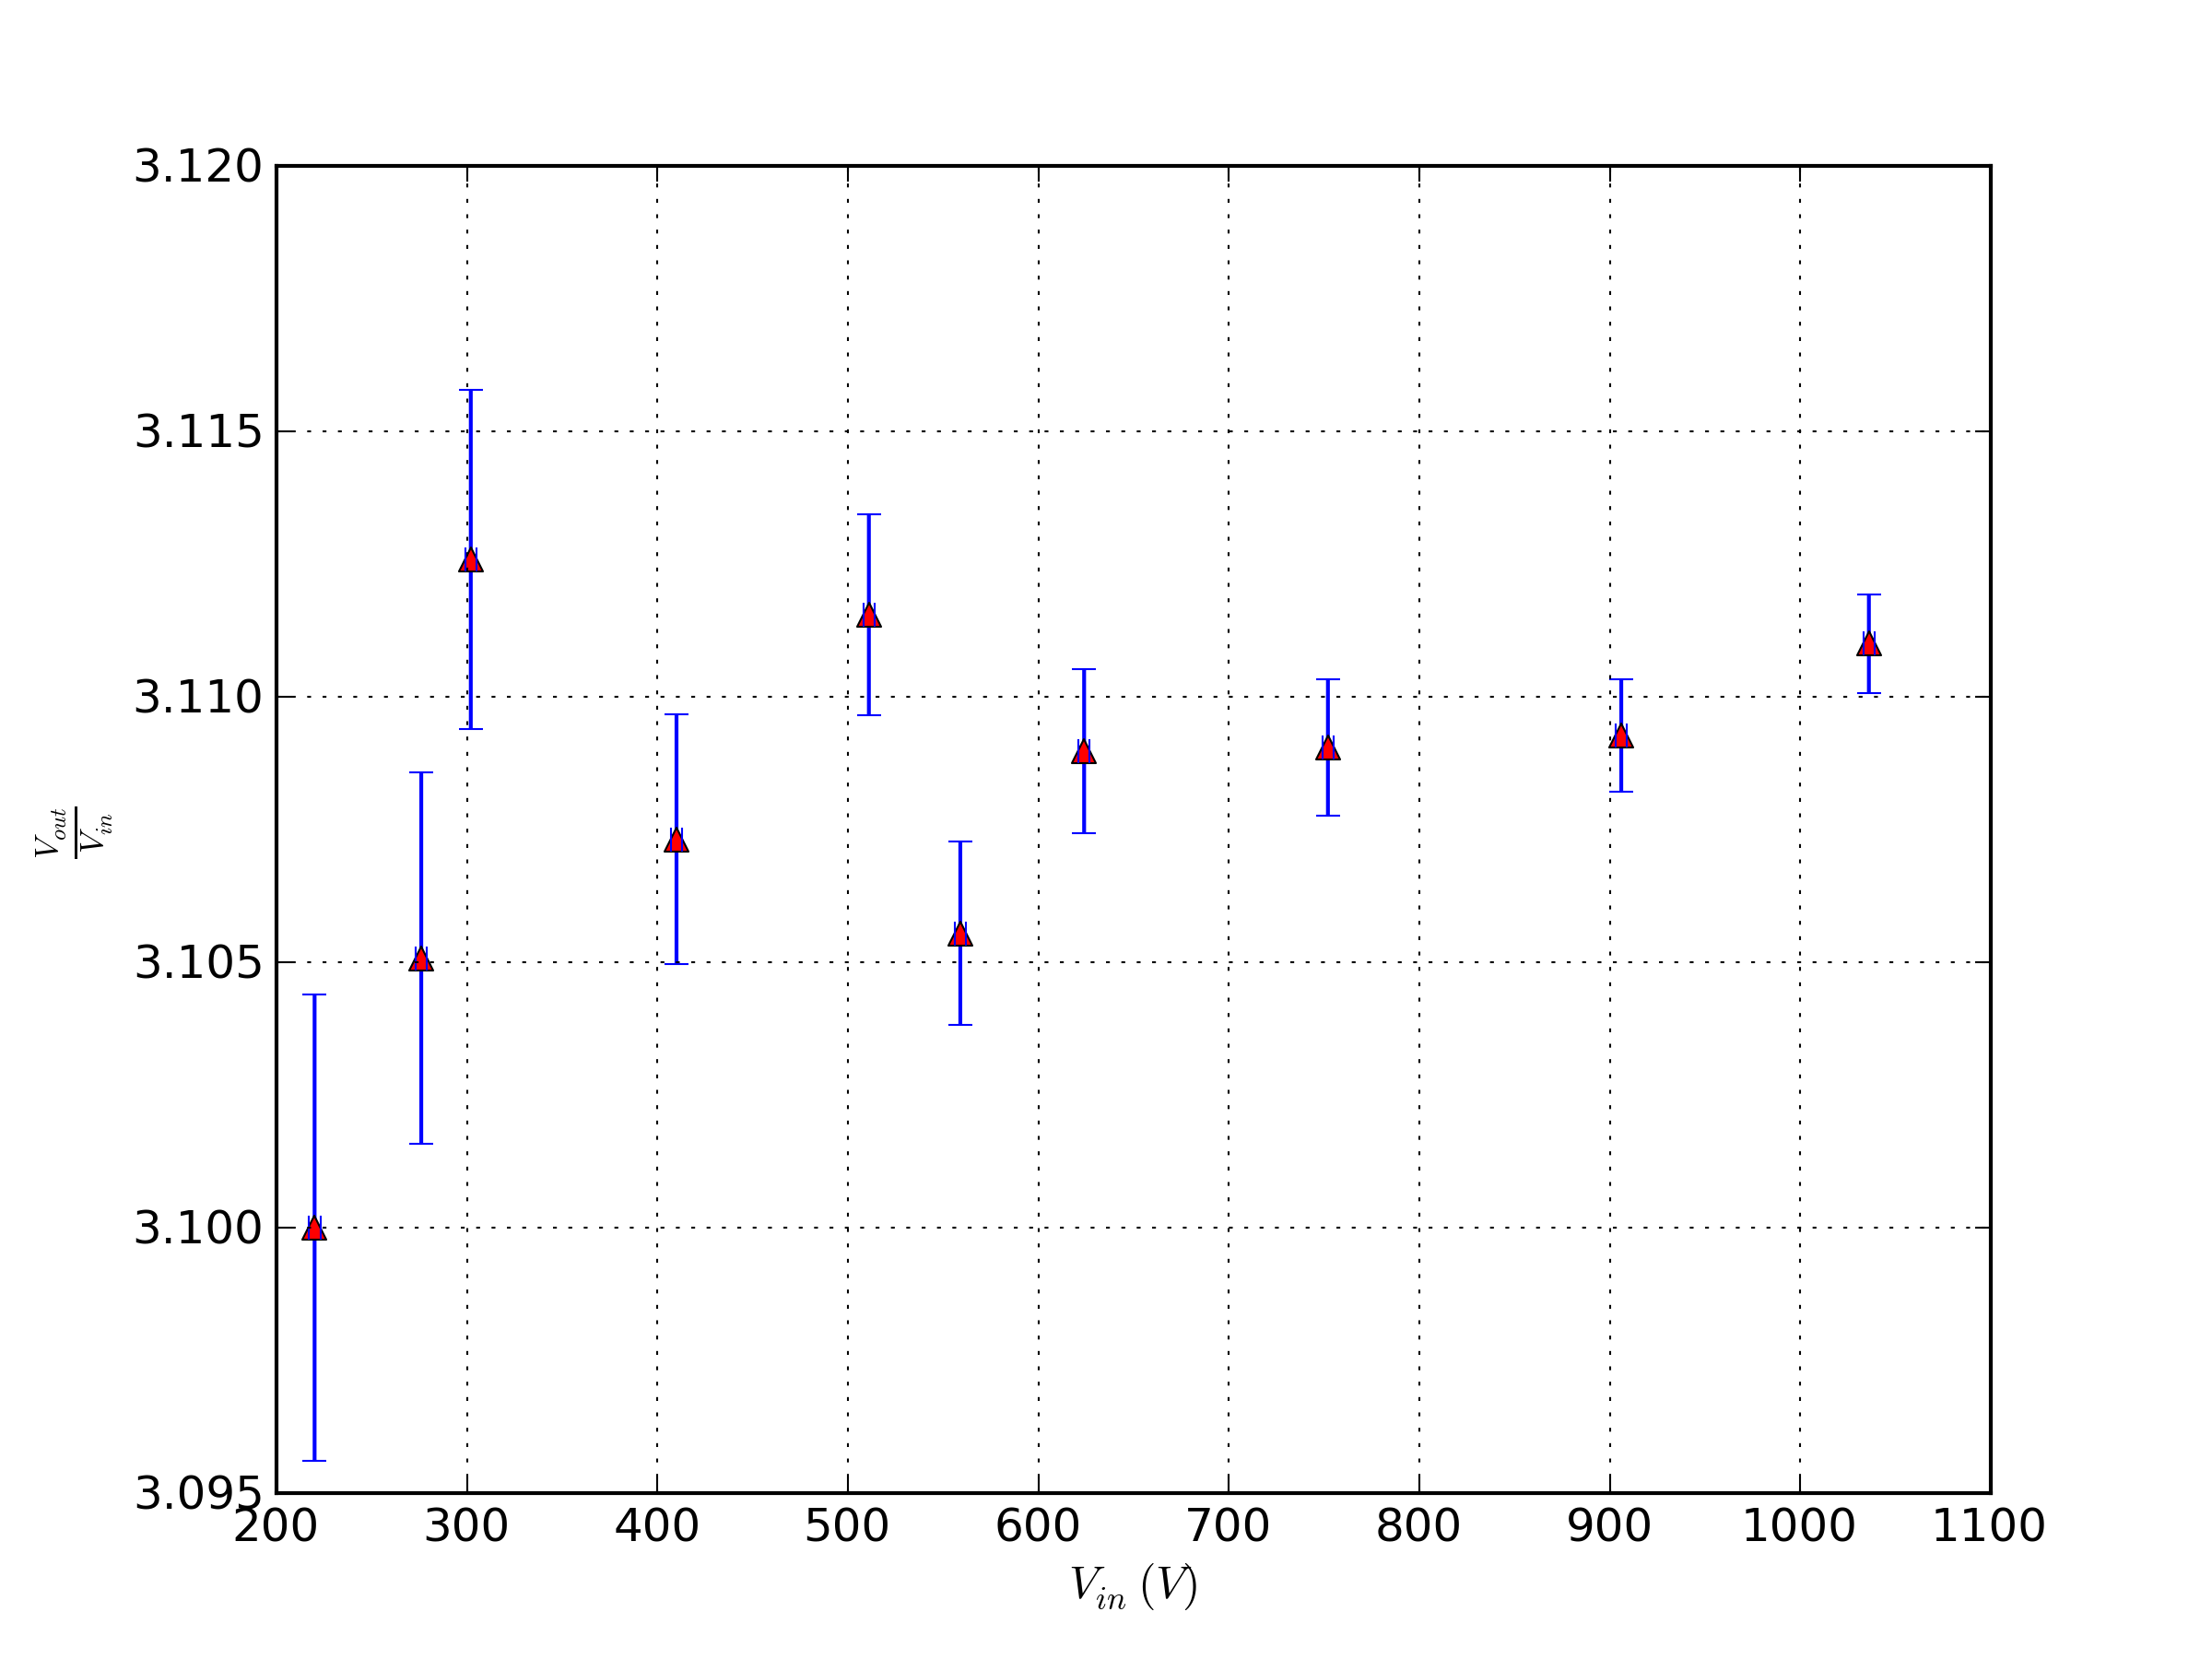
\includegraphics[scale=0.75]{grafici/C1/part22.png}


\begin{center}
\begin{tabular}{*{4}{c}}
Corrente1($nA$) & Potenziale1($mV$) & Corrente2($nA$) & Potenziale2($mV$)\\
\midrule
2.378 & 201 & 3043 & 207\\
2.500 & 261 & 3667 & 250\\
2.972 & 360 & 4703 & 319\\
3.290 & 454 & 6365 & 432\\
4.262 & 574 & 8984 & 609\\
4.856 & 633 & 12326 & 836\\
5.640 & 794 & 16898 & 1145\\
5.090 & 925 & 340 & 24\\
1971 & 1005 & 725 & 50\\
2290 & 1168 & 966 & 66\\
2524 & 1286 & 1595 & 108\\
2850 & 1454 & 1822 & 124\\
3116 & 1589 & 2160 & 146\\
3407 & 1737 & 2302 & 157\\
3883 & 1980 & 2584 & 176\\
4229 & 2157 & 3100 & 211\\
4598 & 2344 & 3370 & 229\\
5072 & 2586 & 4036 & 274\\
5505 & 2807 & 4348 & 295\\
5820 & 2967 & 4596 & 312\\
6257 & 3191 & 4894 & 332\\
6738 & 3436 & 5578 & 379\\
7521 & 3835 & 6613 & 449\\
7880 & 4018 & 6963 & 473\\
8493 & 4331 & 7371 & 500\\
8852 & 4514 & 7864 & 533\\
9135 & 4658 & 8603 & 584\\
9431 & 4809 & 9066 & 615\\
9720 & 4957 & 9667 & 656\\
9972 & 5085 & 10816 & 733\\

\end{tabular}
\end{center}


